\documentclass[xcolor=dvipsnames,notes=hide]{beamer}
%\documentclass[notes=only]{beamer}
%\documentclass[xcolor=dvipsnames, notes=hide]{beamer} 
\usepackage{ulem}
\usepackage{tabularx}
\usepackage{xcolor,colortbl}
\usepackage{pgfpages}

\newcommand{\mc}[2]{\multicolumn{#1}{c}{#2}}
\definecolor{Gray}{gray}{0.85}
\definecolor{LightGreen}{rgb}{1,0.88,1}

\newcolumntype{a}{>{\columncolor{Gray}} X }
\newcolumntype{b}{>{\columncolor{white}} X }

\usepackage{default}
\usepackage{pgfpages} %This is needed for notes presentation!
\setbeameroption{show notes on second screen=left}
\usepackage{soul}
\usepackage[czech]{babel}
\usepackage[utf8]{inputenc}
\usepackage{hyperref}
\hypersetup{colorlinks,linkcolor=NavyBlue,urlcolor=NavyBlue}
\usepackage{times}



\pgfdeclareimage[height=1.cm]{conference-logo}{images/dasenka.jpg}
\logo{\pgfuseimage{conference-logo}}

\title{Sdílené intelektuální spoluvlastnictví}

\subtitle{Proč je open source software na okraji?}

\author[J. Čepický] % (optional, use only with lots of authors)
{Jáchym~Čepický\inst{1}}
% - Give the names in the same order as the appear in the paper.
% - Use the \inst{?} command only if the authors have different
%   affiliation.

\institute % (optional, but mostly needed)
{
  \inst{1}%
  \url{http://les-ejk.cz}, \url{http://osgeo.cz}\\
}
  
% - Use the \inst command only if there are several affiliations.
% - Keep it simple, no one is interested in your street address.

\date[Geoinformatics 2014] % (optional, should be abbreviation of conference name)
{Geoinformatics 2014}
% - Either use conference name or its abbreviation.
% - Not really informative to the audience, more for people (including
%   yourself) who are reading the slides online



\begin{document}

%\begin{abstract}
%\end{abstract}

\begin{frame}
\titlepage

\note{Dobrý den}
\end{frame}

\begin{frame}\begin{center}
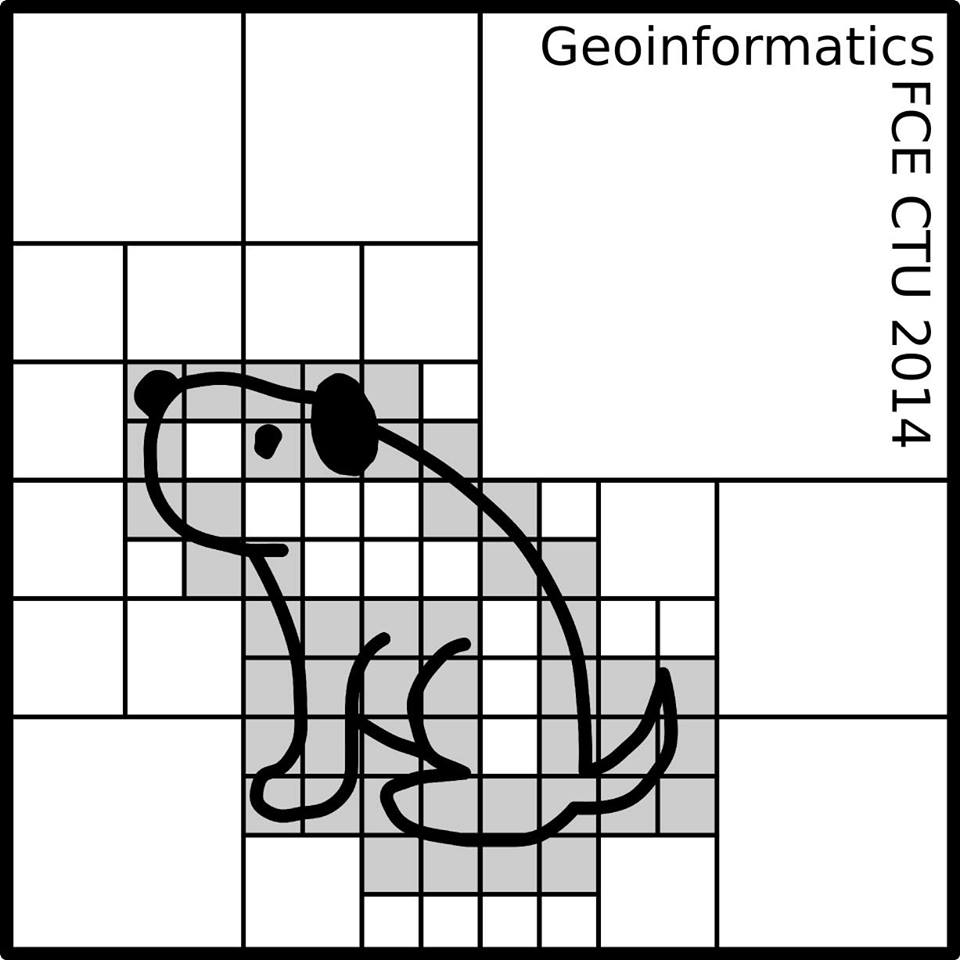
\includegraphics[width=0.4\textwidth]{images/dasenka.jpg}
\note{
    vystupuju zde na tradiční akci Geoinformatics, která je pro mě hlavní českou
    akcí se zaměřením na free a open source software pro geoinformatiku. Já se
    otevřeným software zabývám přibližně od roku 2002 a přibližně také od té doby se
    datuje moje zapojení se do komunity nejdříve uživatelů a později vývojářů. Za ty
    roky jsem viděl několik věcí, které mě nutí k několika myšlenkám, o které bych
    se s vámi rád podělil.
}
\end{center}\end{frame}

%%%%%%%%%%%%%%%%%%%%%%%%%%%%%%%%%%%%%%%%%%%%%%%%%%%%%%%%%%%%%%%%%%%%%%%%%%
\begin{frame}\begin{center}
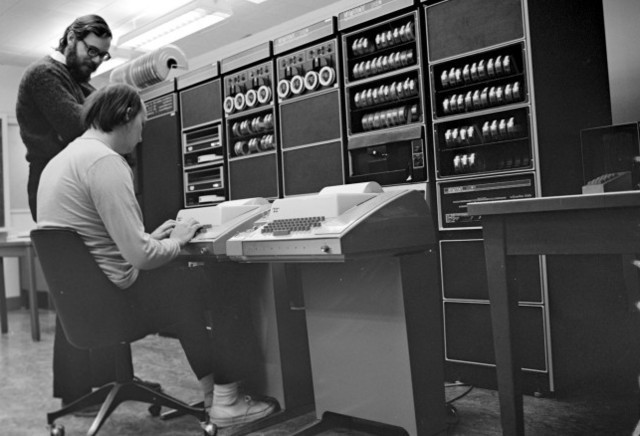
\includegraphics[width=0.7\textwidth]{images/unix-coders.jpg}
\note{
    Asi víte, že staří programátoři mezi sebou sdíleli zdrojový kód programů zcela
    běžně - nikdo nepovažoval za nutné se tím zaobírat a asi nikoho nenapadlo, že se
    jedná vlastně o důležitou svobodu, kterou je potřeba bránit. Najednou byli v
    situaci, kdy se okolo nich zdrojové kódy zavíraly a to co bylo dříve veřejným
    statkem se stalo soukromým vlastnictvím, jakkoliv se mi do dnes nezdá,
    že si někdo dělá nárok na vlastnictví myšlenky.
}
\end{center}\end{frame}
%%%%%%%%%%%%%%%%%%%%%%%%%%%%%%%%%%%%%%%%%%%%%%%%%%%%%%%%%%%%%%%%%%%%%%%%%%
\begin{frame}\begin{center}
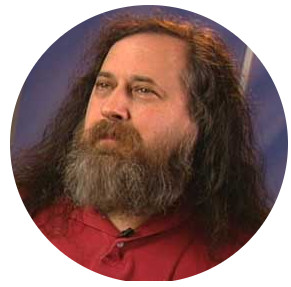
\includegraphics[width=0.5\textwidth]{images/rms.jpg}
\note{
    Situaci si uvědomil Richard Metthew Stallman a rozhodl se ji řešit s razancí pro
    něj asi typickou. V 80. letech založil Free Software Foundation. Většina z vás
    asi zná přibližně příběh operačního systému GNU, který v 90 letech využil jádro
    Linux a spolu s ním funguje do dnes v různých tzv. linuxových distribucích.
}
\end{center}\end{frame}
%%%%%%%%%%%%%%%%%%%%%%%%%%%%%%%%%%%%%%%%%%%%%%%%%%%%%%%%%%%%%%%%%%%%%%%%%%
\begin{frame}\begin{center}
\includegraphics<1>[width=0.5\textwidth]{images/super-linux.jpg}
\only<2>{
\begin{itemize}
    \item číst
    \item distribuovat
    \item měnit a změny dále distribuovat
\end{itemize}
}
\note<1>{
Dnes je Linux nejpoužívanějším serverovým operačním systémem, používá se v
mobilních zařezních, na super počítačích. Proč se tak stalo? Protože je to
otevřený systém
}
\note<2>{
\begin{itemize}
    \item systém,  ve kterém ostatní sdílí svůj kód - svoje know-how - svoje
  intelektuální vlastnictví s ostatními.
    \item to se stalo díky licenci, která umožňuje sdílet práci jednotlivce bez obav, že
  by ji v budoucnu někdo uzavřel 
\end{itemize}
}
\end{center}\end{frame}

%%%%%%%%%%%%%%%%%%%%%%%%%%%%%%%%%%%%%%%%%%%%%%%%%%%%%%%%%%%%%%%%%%%%%%%%%%
\begin{frame}\begin{center}
\begin{itemize}
    \item zkoumej
    \item publikuj, opakovatelným způsobem
    \item ověření na jiném pracovišti
\end{itemize}
\note{
Ale koncept sdílení není přece vynalezen v 80 letech. Západní věda tak jak ji
chápeme je snad od dob antiky postavena na stejných principech: publikuji
výsledek způsobem, že je opakovatelný, očekávám, že někdo jiný mou práci
zopakuje, přezkouší její platnost, případně navrhne některé změny, a výsledek
opět publikuje. Vědecká komunita díky sdílení informací posouvá hranice našeho
poznání dále, stejně jako komunita vývojářská posouvá hranice software.
}
\end{center}\end{frame}


%%%%%%%%%%%%%%%%%%%%%%%%%%%%%%%%%%%%%%%%%%%%%%%%%%%%%%%%%%%%%%%%%%%%%%%%%
\begin{frame}\begin{center}
\includegraphics<1>[width=0.5\textwidth]{images/wikipedia.jpg}
\includegraphics<2>[width=0.5\textwidth]{images/osm-logo.png}
\note{
Open source software není jediný příklad pro fungující intelektuální
spoluvlastnictví. Nikdo snad nepochybuje, že wikipedia je spolehlivý informační
zdroj a přitom na její obsah nemá nikdo monopol, neexistuje globální autorita,
která by strážila věcný obsah Wikipedie.\textbf{NEXT}\\
~\\
OpenStreetMap je podle mě další úspěšný
projekt. Jako geoprostoroví profesionálové můžete zpochybňovat polohovou
přesnost dat, jejich faktickou správnost nebo aktuálnost, ale nemůžete
zpochybnit, že globálně vzato je to ucelený dataset který nemá v prorietárním
světe obdoby. Nově vziklá služba Mapillary umožňuje uživatelům nahrávat fotky s
geolokací a vytvořit tak pomocí "crowdu" alternativu ke službě google street
view.
}
\end{center}\end{frame}

%%%%%%%%%%%%%%%%%%%%%%%%%%%%%%%%%%%%%%%%%%%%%%%%%%%%%%%%%%%%%%%%%%%%%%%%%%
\begin{frame}\begin{center}
\begin{itemize}
    \item číst
    \item sdílet
    \item měnit a změny dále distribuovat
\end{itemize}
\note{
Všechny tyto příklady mají díky svým licencím společné tři základní vlastnosti,
které vyzývají další a další uživatele aby se přidali: vidět obsah, sdílet obsah
a provádět změny v obsahu a sdílet tyto změny dál.
}
\end{center}\end{frame}

%%%%%%%%%%%%%%%%%%%%%%%%%%%%%%%%%%%%%%%%%%%%%%%%%%%%%%%%%%%%%%%%%%%%%%%%%
\begin{frame}\begin{center}

\includegraphics[width=0.7\textwidth]{images/internet.jpg}
\note{
Dalším důvodem je rozmach sítě internet - technologicky neutrální a otevřené
technologie, spojující lidi. Bez internetu by nebyla ani wikipedie, ani open
streetmap, ani většina open source software. 
}
\end{center}\end{frame}
%%%%%%%%%%%%%%%%%%%%%%%%%%%%%%%%%%%%%%%%%%%%%%%%%%%%%%%%%%%%%%%%%%%%%%%%%
\begin{frame}\begin{center}
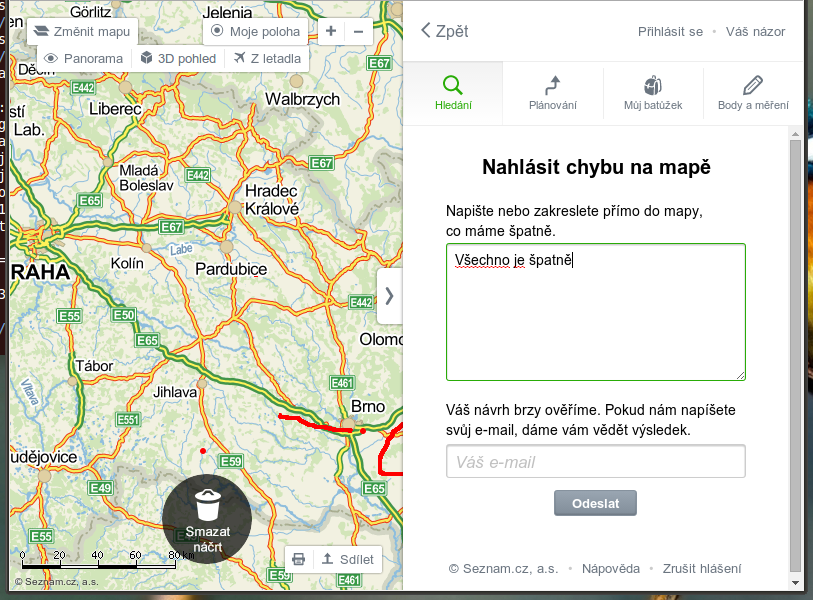
\includegraphics[width=0.6\textwidth]{images/seznam.png}
\note{
Praktický příklad kdy sdílení intelektuálního vlastnictví nevede ke sdílenému
intelektuálnímu spoluvlastnictví: Není to, že můžete opravit data Seznamu v jeho
mapách tak trochu asymetrický vztah? Proč by někdo systematicky pomáhal zadarmo
upravit data soukromému subjektu, který je ale dále nesdílí? Pro takové
pomocníky mám tip: potřeboval bych posekat vyvézt žumpu, sice z toho asi
nebudete mít žádný přímý užitek a já vám vaši žumpu vyvézt nepůjdu, ale může vás
hřát pocit, že jste mi pomohli, já budu opravdu moc rád.
}
\end{center}\end{frame}
%%%%%%%%%%%%%%%%%%%%%%%%%%%%%%%%%%%%%%%%%%%%%%%%%%%%%%%%%%%%%%%%%%%%%%%%%
\begin{frame}\begin{center}
\note{
Uvedl jsem minimálně dva úspěšné crowd-sourcingové projekty (wikipedii,
openstreetmap).  Já si ale myslím, že open source software je příkladem selhání
tohoto - crowdsource - modelu.  Důvody prototo mé tvrzení jsou následující:
}
\end{center}\end{frame}
%%%%%%%%%%%%%%%%%%%%%%%%%%%%%%%%%%%%%%%%%%%%%%%%%%%%%%%%%%%%%%%%%%%%%%%%%
\begin{frame}\begin{center}
\includegraphics<1>[width=0.7\textwidth]{images/market-share.jpg}
\includegraphics<2>[width=0.7\textwidth]{images/win-to-linux.jpg}
\note<1>{
Open Source jako platforma má sice vysoký podíl zastoupení na superpočítačích a
serverech obecně, nepodařilo se mu etablovat se na desktopech. Podle wikipedie
má momentálně 1.62\% desktopů.
}
\note<2>{
S každou další obměnou Windows můžeme číst, jaká je to ohromná příležitost pro
Linux na destopech [1][2], abychom se za rok opět divili, že se tomu tak
nestalo.
}
\end{center}\end{frame}
%%%%%%%%%%%%%%%%%%%%%%%%%%%%%%%%%%%%%%%%%%%%%%%%%%%%%%%%%%%%%%%%%%%%%%%%%
\begin{frame}\begin{center}

\includegraphics[width=0.7\textwidth]{images/android-linux.png}
\note{
Pokud už někdo používá Open Source produkty (produkty Open Source vývoje),
většinou ani netuší, že tak činí. Najdou se i tací, kteří mají telefon s
androidem atd a budou tvrdit, že OSS model vývoje nemůže fungovat. Lidi nejenom
že nezajímá, jaká rizika jsou spojena s užíváním OSS nebo proprietárního
software, oni netuší, že tyto dva světy existují.
}
\end{center}\end{frame}
%%%%%%%%%%%%%%%%%%%%%%%%%%%%%%%%%%%%%%%%%%%%%%%%%%%%%%%%%%%%%%%%%%%%%%%%%%
\begin{frame}\begin{center}

\includegraphics[width=0.7\textwidth]{images/cyanogen.jpg}
\note{
Pokud Android zažívá nebývalý boom, můžeme se navzájem poplácávat po ramenou,
jak to ten Linux těm proprietárním operačním systémům natírá, ale ve skutečnosti
je to jeho největší prohra: že jádro je Linux  zajímá jenom technologické geeky.
Zatím co sehnat proprietární aplikaci na běžné linuxové distro je spíše výjimka,
veškerý ekosystém aplikací v mobilních telefonech je proprietární (čest
výjimkám). Nic na tom nemění ani to, že Android je skutečně open source a můžete
si na telefon nainstalovat např. cyanogen mod (alternativní distribuci androidu)
- většina lidí to neví a je jim to jedno.  Open source model selhal, neumí sám
sebe prodat z pohledu uživatelské masy.
}
\end{center}\end{frame}
%%%%%%%%%%%%%%%%%%%%%%%%%%%%%%%%%%%%%%%%%%%%%%%%%%%%%%%%%%%%%%%%%%%%%%%%%%
\begin{frame}\begin{center}
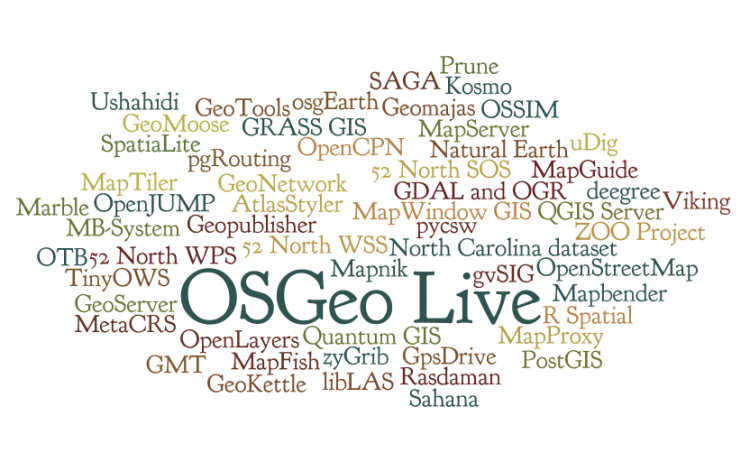
\includegraphics[width=0.7\textwidth]{images/750px-Osgeolive_wordle.png}
\note{
To samé platí pro Open Source GIS. Ty programy jsou tu, fungují, jsou tu někdy i
desítky let, stále žijí, rozvíjí se jejich komunita - vývojářská i uživatelská.
Přesto, když přijdu do státní instituce a začnu mluvit o open source
alternativách narazím. 
}
\end{center}\end{frame}
%%%%%%%%%%%%%%%%%%%%%%%%%%%%%%%%%%%%%%%%%%%%%%%%%%%%%%%%%%%%%%%%%%%%%%%%%
\begin{frame}\begin{center}
\begin{itemize}
\item Opravdu to funguje?
\item Never touch running system.
\item Podpora.
\end{itemize}
\note{
Narazím i v případě, že proprietární stávající řešení objektivně v nějakém svém
bodě selhává a já nabízím open source alternativu. Bylo by to na delší výzkum,
ale opakuje se následující:
\begin{itemize}
\item Neurčitě vyjádřená obava z toho, jestli to opravdu funguje
\item Změna by byla problematická
\item Nemá kdo by nás podporoval
\end{itemize}
}
\end{center}\end{frame}
%%%%%%%%%%%%%%%%%%%%%%%%%%%%%%%%%%%%%%%%%%%%%%%%%%%%%%%%%%%%%%%%%%%%%%%%%%
\begin{frame}\begin{center}
\includegraphics<1>[width=0.7\textwidth]{images/good.png}
\includegraphics<2>[width=0.5\textwidth]{images/angry-computer-meme.png}
\note<1>{
Jak to, že lidi zahodili Britaniku a další tištěné encyklopedie a hromadně
začali používat wikipedii jako primární zdroj pro své často vědecké práce - a
nikomu to nevadí? Jak to, že lidi mají OSM ve svých navigacích a to i přes
objektivní nedostatky, která tato data mají pro něco tak základního, jako je
navigace v autech (mám na mysli např. jednosměrné ulice, rychlostní omezení)?
}
\note<2>{A
jak to, že i přes to lidi stejně samozřejmě nezačnou používat open source
software?
}
\end{center}\end{frame}
%%%%%%%%%%%%%%%%%%%%%%%%%%%%%%%%%%%%%%%%%%%%%%%%%%%%%%%%%%%%%%%%%%%%%%%%%
\begin{frame}\begin{center}
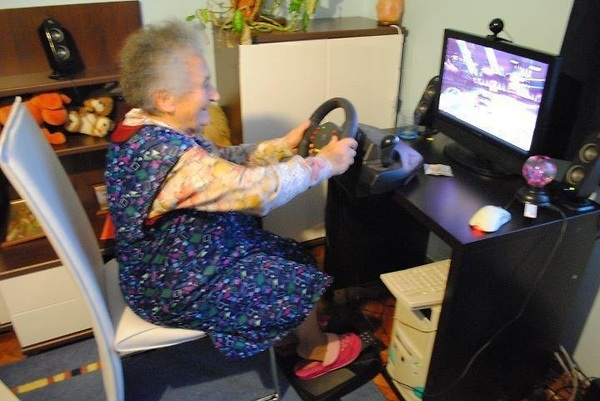
\includegraphics[width=0.7\textwidth]{images/aaa-A-super-grandma-playing-NFS.jpg}
\note{
Moje tchýně - tedy babička mých dětí - bez technického vzdělání, jejíž user
experience se opírá hlavně o to, aby si mohla spustit browser a jít na záložku
seznam.cz, již dva roky používá Ubuntu Linux a spontánně projevuje známky
spokojenosti.
}
\end{center}\end{frame}
%%%%%%%%%%%%%%%%%%%%%%%%%%%%%%%%%%%%%%%%%%%%%%%%%%%%%%%%%%%%%%%%%%%%%%%%%%
\begin{frame}\begin{center}

\includegraphics[width=0.7\textwidth]{images/burger-takeaway.png}
\note{
Řekl bych, že open source software je celkem známý v oblasti firem v oboru. Mám
pocit, že jak je někde veřejná správa, bere se automaticky proprietární řešení.
Bez analýzy. Prostě vezme co je u ruky.\\

~\\
K jednotlivým bodům proč se nepoužívá open source GIS software:
}
\end{center}\end{frame}
%%%%%%%%%%%%%%%%%%%%%%%%%%%%%%%%%%%%%%%%%%%%%%%%%%%%%%%%%%%%%%%%%%%%%%%%%%
\begin{frame}\begin{center}

\includegraphics[width=0.7\textwidth]{images/hd_computer_guy_meme_by_zapgod16-d4t2jh3.png}
\note{
\textbf{Neurčitě vyjádřená obava z toho, zda-li to opravdu funguje}\\
~\\
Používám to, co jsem se naučil, co jsem poznal do svých 35 let. Open Source
software se začal prosazovat v 90. letech, open source GIS až od roku 2000. Do
výuky ho do dnes většina českých fakult zařazuje pouze okrajově (pokud vůbec).
No a bojíte se toho, co neznáte a nepřesvědčí vás to, že někdo jiný, kdo už
přeplaval na druhý břeh říká, že to funguje.
}
\end{center}\end{frame}
%%%%%%%%%%%%%%%%%%%%%%%%%%%%%%%%%%%%%%%%%%%%%%%%%%%%%%%%%%%%%%%%%%%%%%%%%%
\begin{frame}\begin{center}
\includegraphics<1>[width=0.4\textwidth]{images/venere_botticelli_volto_max_by_freddyorsini-d6esi66.jpg}
\includegraphics<2>[width=0.4\textwidth]{images/hqdefault.jpg}
\includegraphics<3>[width=0.4\textwidth]{images/venere_botticelli_volto_max_by_freddyorsini-d6esi66.jpg}
\includegraphics<4>[width=0.4\textwidth]{images/botticelli_birth_venus_2.jpg}
\note{
\textbf{Změna je problematická}\\
~\\
Změna vždycky bolí. Smyslem prosazování open source gis není porazit
proprietární software nebo ho vytlačit. Představte si, že přijdete do organizace
řeknete, že nasadíte Open Source, abyste z tohohle \textbf{NEXT} dostali tohle.
Ale z praxe spíš \textbf{NEXT} tohle. Než to odladíte\textbf{NEXT}.
}
\end{center}\end{frame}
%%%%%%%%%%%%%%%%%%%%%%%%%%%%%%%%%%%%%%%%%%%%%%%%%%%%%%%%%%%%%%%%%%%%%%%%%
\begin{frame}\begin{center}
\includegraphics<1>[width=0.4\textwidth]{images/stock-photo-21408703-modelling-clay-ball.jpg}
\includegraphics<2>[width=0.4\textwidth]{images/puzzle-pieces-2.jpeg}
\note<1>{
Ale pokud bude jakákoliv organizace
držet propritární linku, dostane se do tzv. vendor locku, kdy jakákoliv změna
jediné komoponenty v celém systému nebude možná. Pokud je systém postaven
špatně, nemodulárně, je změna objektivně nemožná.}
\note<2>{Čili prvním krokem je
zmodularizovat systém. Nebo provézt úkrok stranou a na nových projektech
testovat nasazení open source software -- technik jak začít s novou technologií
je více. Pomůže ale, pokud v organizaci existuje někdo, kdo to dělat chce. 
}
\end{center}\end{frame}
%%%%%%%%%%%%%%%%%%%%%%%%%%%%%%%%%%%%%%%%%%%%%%%%%%%%%%%%%%%%%%%%%%%%%%%%%%
\begin{frame}\begin{center}
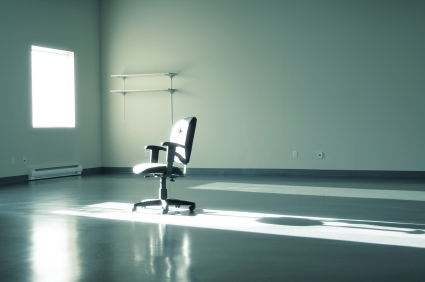
\includegraphics[width=0.6\textwidth]{images/empty-office.jpg}
\note{
\textbf{Nemá nás kdo podporvat}\\
~\\
Absence telefonního čísla je stálý problém. My open soursaři jsme stále
překvapeni z toho, jak se lidi bojí mailing listu. Stackoverflow to trochu řeší,
ale pořád to není ono. A čím je instituce větší, tím je uživatel - odpovědná
osoba - nervóznější z toho, že se namá na koho obrátit, kdyby nastal problém. Je
tu přeci komunita, ta vás podrží ... no, ale vysvětlete to někomu, kdo nedostane
odpověď ani na placené podpoře.
}
\end{center}\end{frame}
%%%%%%%%%%%%%%%%%%%%%%%%%%%%%%%%%%%%%%%%%%%%%%%%%%%%%%%%%%%%%%%%%%%%%%%%%%
\begin{frame}\begin{center}

\includegraphics[width=0.6\textwidth]{images/angry-computer-meme.png}
\note{
Mno. Ale jak to, že chybějící redakce nevadí nikomu v používání wikipedie? U
OpenStreetMap už jsou lidi opatrnější. Už padají dotazy na přesnost dat, na
trolly. Ale přesto je to uznávaný datový zdroj. U Open Source Software je to
pořád něco, co vzbuzuje strach. 
}
\end{center}\end{frame}
%%%%%%%%%%%%%%%%%%%%%%%%%%%%%%%%%%%%%%%%%%%%%%%%%%%%%%%%%%%%%%%%%%%%%%%%%%
\begin{frame}\begin{center}
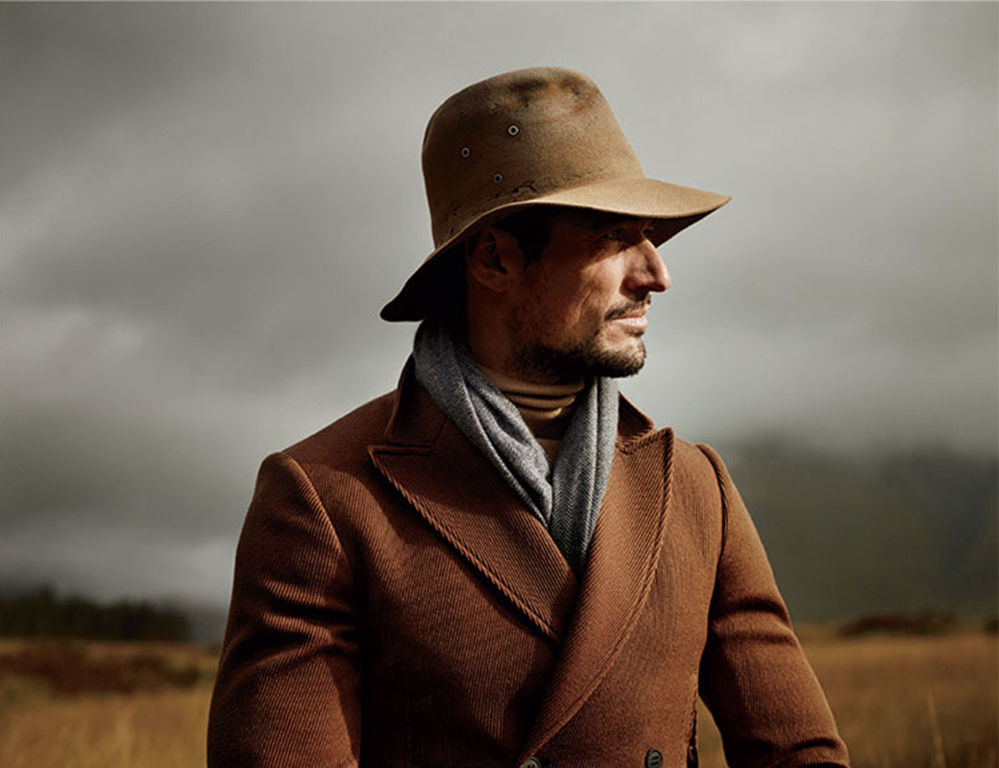
\includegraphics[width=0.6\textwidth]{images/David-Gandy-by-John-Balsom-A-New-Frontier-Man-of-the-World-DerriusPierreCom-3.jpg}
\note{
Mimochodem, kdo kdeska vlastně používá open source software? Kde se dozvěděl o
open source software pro GIS, kteří jsme dnes v produktivním věku a považujeme
se za GIS profesionály? Nadšenci, kteří hledají řešení svého problému a
proprietární software nemohou používat (z licenčních, platformních, systémových
nebo jiných důvodu) nebo zjistili, že řešení jejich
problému neobsahuje. Tedy profíci, kteří hledají řešení svého problému mimo
zaběhlé nebo naučené koleje. No a pomalu nastupující generace profesionálů,
kteří dostali to správné všeobecné vzdělání.
}
\end{center}\end{frame}
%%%%%%%%%%%%%%%%%%%%%%%%%%%%%%%%%%%%%%%%%%%%%%%%%%%%%%%%%%%%%%%%%%%%%%%%%
\begin{frame}\begin{center}
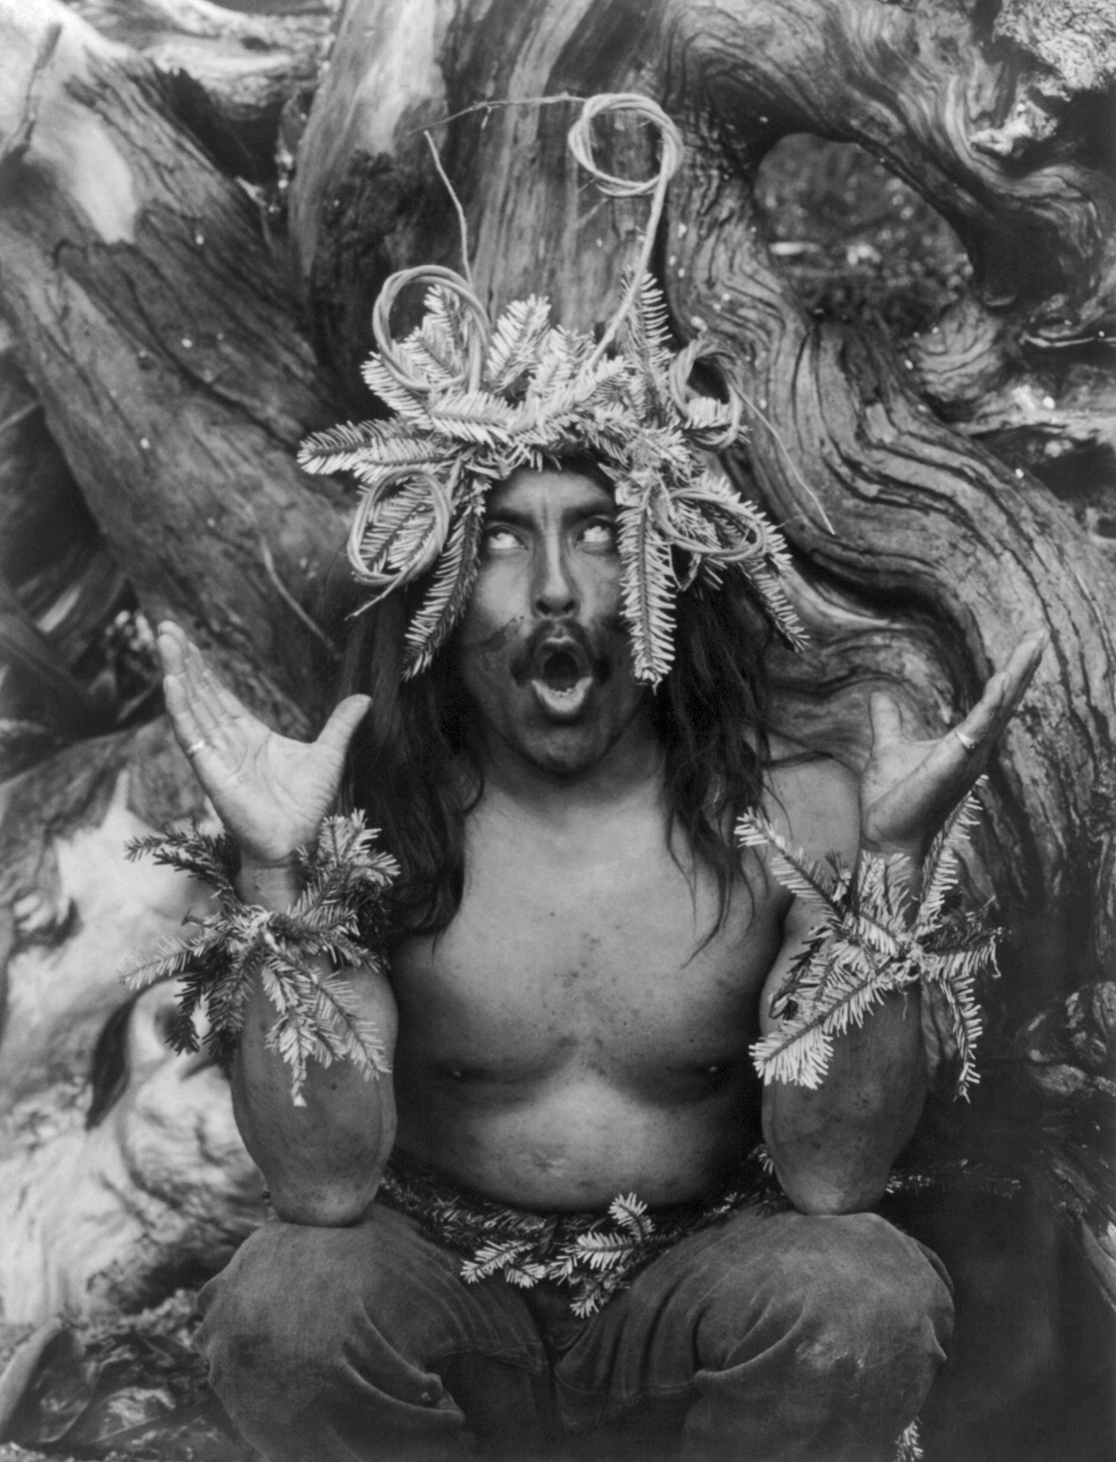
\includegraphics[width=0.6\textwidth]{images/Hamatsa_shaman2.jpg}
\note{
Pořád tady ale brousím kolem toho, že open knowledge - tedy například wikipedia
- open data - tedy například openstreetmap ale celé hnutí za otevřená data,
které nabývá na síle i v ČR jsou ve srovnání s open source software daleko více
společensky přijetelné. Programovaní je asi šamanismus, ke kterému ostatní
přistupují jako k woodoo a věří tomu, co jim kmenový šaman nakuká.
}
\end{center}\end{frame}
%%%%%%%%%%%%%%%%%%%%%%%%%%%%%%%%%%%%%%%%%%%%%%%%%%%%%%%%%%%%%%%%%%%%%%%%%%
\begin{frame}\begin{center}

\includegraphics[width=0.6\textwidth]{images/hand-shake-vector-eps-illustration-30954827.jpg}
\note{
Rád bych ale zde na této konferenci vyzval zástupce openstreetmap a wikipedie k
užší spolupráci minimálně v otevřené geo- oblasti. Vy víte, že bez otevřenéného
přístupu by ani vaše projekty nebyly možné. Uvědomujete si, že i pro vaše
projekty a iniciativy je open source software přímo životně důležitý. Rád bych
vyjádřil, jakou radost cítím, že jsme se tady na Geoinformatics konečně sešli
alespoň s větším množstvím zástupců z OpenStreetMap.
}
\end{center}\end{frame}
%%%%%%%%%%%%%%%%%%%%%%%%%%%%%%%%%%%%%%%%%%%%%%%%%%%%%%%%%%%%%%%%%%%%%%%%%%
\begin{frame}\begin{center}
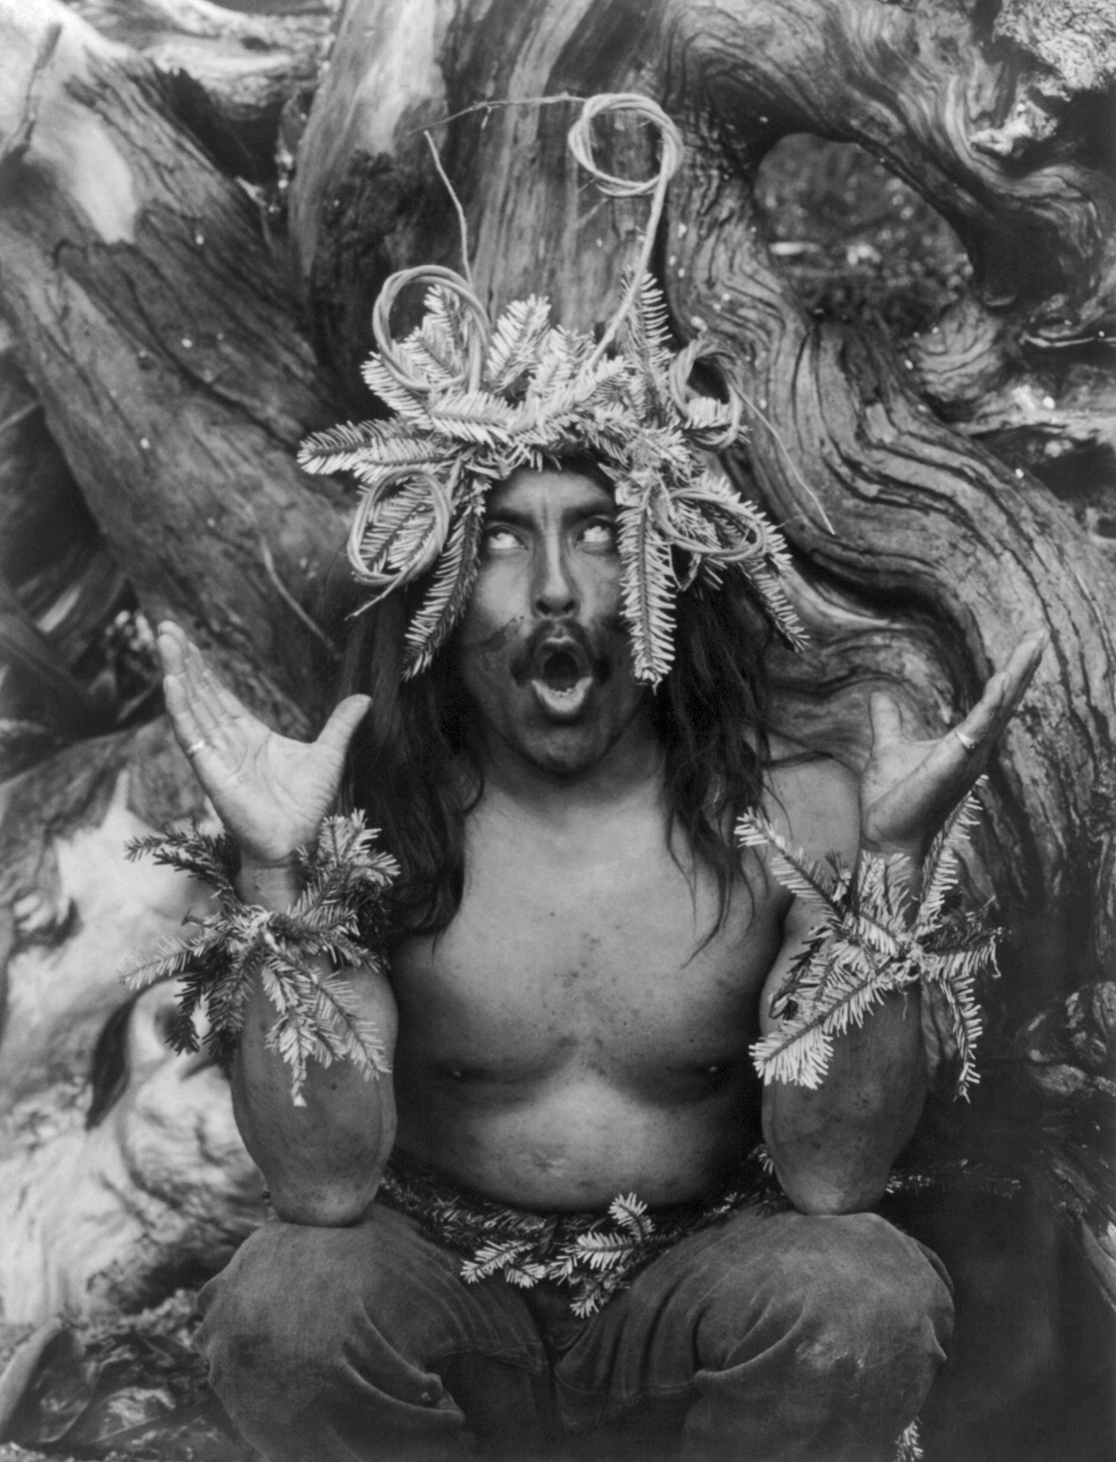
\includegraphics[width=0.6\textwidth]{images/Hamatsa_shaman2.jpg}
\note{
Otevřenost - žít otevřený život v otevřené společnosti - nelze oddělit. Nemá
cenu si vybírat, že v nějakém aspektu budete otevření a v jiném ne. Neberte mě
za slovo - i já mám telefon s Androidem a několik nakoupených aplikací. Bavím se
o ideálu, o způsobu myšlení, o způsobu přemýšlení o sdíleném intelektuálním
spoluvlastnictví. Kmenoví šamani se společnosti snaží nakukat, že sdílené
intelektuální spoluvlastnictví je tabu. Přitom je to vlastně docela přirozené a
staré jako lidstvo samo.
}
\end{center}\end{frame}
%%%%%%%%%%%%%%%%%%%%%%%%%%%%%%%%%%%%%%%%%%%%%%%%%%%%%%%%%%%%%%%%%%%%%%%%%
\begin{frame}\begin{center}
\note{
Otevřenost dat, znalostí a software totiž není samozřejmá společenská kvalita,
je nekončící proces, za který má smysl se brát. A pokud se vám jako GISákům
někdo směje a říká, "jenom se z toho ne FOSSer", berte to s humorem - vy jste
profík, který překročil čáru a zajímá se o to, co je za obzorem, šel na průzkum,
objevuje nové světy. K takové cestě patří neslavný návrat domů, ale v srdci si
tu cestu nesete s sebou. On sedí ve své zaprděné díře, dál se nedostal, a
poslouchá kmenového šamana.
}
\end{center}\end{frame}

%%%%%%%%%%%%%%%%%%%%%%%%%%%%%%%%%%%%%%%%%%%%%%%%%%%%%%%%%%%%%%%%%%%%%%%%%%
\section*{Závěr}
\begin{frame}\begin{center}
    Dotazy?\\

    \vfill

    \url{http://osgeo.cz}

    \vfill
    
\includegraphics[width=0.15\textwidth]{images/cc.png}

\note{Tato prezentace je samozřejmě uvolněna pod licencí Creative Commons,
Uveďte autora. \\
~\\
Děkuji Vám za pozornost, kterou jste mi věnovali a jsem připraven
čelit vašim dotazům, máte-li nějaké}
\end{center}\end{frame}


\end{document}
